\documentclass[12pt,letterpaper]{article}
\usepackage{fullpage}
\usepackage[top=2cm, bottom=4.5cm, left=2.5cm, right=2.5cm]{geometry}
\usepackage{amsmath,amsthm,amsfonts,amssymb,amscd}
\usepackage{lastpage}
\usepackage{enumerate}
\usepackage{fancyhdr}
\usepackage{mathrsfs}
\usepackage{subcaption} % For subfigures
\usepackage{xcolor}
\usepackage{graphicx}
\usepackage{listings}
\usepackage{hyperref}
\usepackage{tgpagella}
\usepackage{physics}
\usepackage{minted}
% \usepackage{erewhon-math}
% \usepackage{unicode-math}
% \setmathfont{texgyrepagella-math.otf}

\hypersetup{
  colorlinks=true,
  linkcolor=blue,
  linkbordercolor={0 0 1}
}   
 

\lstdefinestyle{Python}{
    language        = Python,
    frame           = lines, 
    basicstyle      = \footnotesize,
    keywordstyle    = \color{blue},
    stringstyle     = \color{green},
    commentstyle    = \color{red}\ttfamily
}

\setlength{\parindent}{0.0in}
\setlength{\parskip}{0.05in}

% Edit these as appropriate
\newcommand\course{MATH-403}
\newcommand\hwnumber{1}                  

\newcommand{\K}{\mathbb{K}}
\newcommand{\R}{\mathbb{R}}
\newcommand{\N}{\mathbb{N}}
\newcommand{\Q}{\mathbb{Q}}
\newcommand{\C}{\mathbb{C}}
\newcommand{\Z}{\mathbb{Z}}
\newcommand{\E}{\Expect}
\renewcommand{\P}{\mathbb{P}}
\newcommand{\ii}{\mathrm{i}}
\newcommand{\cK}{\mathcal K}
\newcommand{\comp}{\mathsf{c}}
\renewcommand{\le}{\leqslant}
\renewcommand{\ge}{\geqslant}
\renewcommand{\labelenumi}{\alph{enumi})}
\newcommand{\jatnote}[1]{\textcolor{medblue}{\textbf{[JAT: #1]}}}
\newcommand{\mnote}[1]{\textcolor{purple}{\textbf{[MU: #1]}}}
\newcommand{\tone}[1]{\textcolor{orange}{\textbf{[Tone?: #1]}}}
\newcommand{\itone}[1]{\textcolor{rust}{\textbf{[Improved tone: #1]}}}

\newcommand{\xmark}{\ding{55}}
\newcommand{\inv}[1]{#1^{-1}}
\newcommand{\F}{\mathbb{F}}
\newcommand{\Msym}{\mathbb{M}_{\rm sym}}
\newcommand{\Mplus}{\mathbb{M}_{+}}


\newcommand{\imag}{\operatorname{Im}}


\newcommand{\eps}{\varepsilon}
\newcommand{\econst}{\mathrm{e}}

\newcommand{\vct}[1]{\bm{#1}}
\newcommand{\mtx}[1]{\bm{#1}}

\newcommand{\onevct}{\mathbf{1}}
\newcommand{\Id}{\mathbf{I}}

% \newcommand{\trace}{\operatorname{tr}}
% \newcommand{\rank}{\operatorname{rank}}
% \newcommand{\range}{\operatorname{range}}
\newcommand{\diag}{\operatorname{diag}}

\newcommand{\dist}{\operatorname{dist}}
% \newcommand{\abs}[1]{\vert #1 \vert}
% \newcommand{\norm}[1]{\Vert #1 \Vert}
\newcommand{\normsq}[1]{\norm{#1}^2}
\newcommand{\fnorm}[1]{\norm{#1}_{\mathrm{F}}}
\newcommand{\snorm}[1]{\norm{#1}_2}
\newcommand{\snormsq}[1]{\snorm{#1}^2}
\newcommand{\triplenorm}[1]{\vert\!\vert\!\vert #1 \vert\!\vert\!\vert}
\newcommand{\precond}[1]{P^{-\frac{1}{2}}(#1) P^{-\frac{1}{2}}}
\newcommand{\RPCPrecond}{\precond{A_\mu}}
\newcommand{\RPC}{\hat A^{(k)}}
% \newcommand{\ip}[2]{\langle #1, \, #2 \rangle}

\newcommand{\lowrank}[2]{\llbracket {#1} \rrbracket_{#2}}

\newcommand{\psdle}{\preccurlyeq}
\newcommand{\psdge}{\succcurlyeq}

\newcommand{\Expect}{\operatorname{\mathbb{E}}}
\newcommand{\Prob}[1]{\mathbb{P}\left\{ #1 \right\}}

\newcommand{\minimize}{\text{minimize}}
\newcommand{\subjto}{\text{subject to}}
\newcommand{\argmin}{\operatorname{arg\,min}}


\pagestyle{fancyplain}
\headheight 35pt
\lhead{Alix \textsc{Benoit}}
\chead{\textbf{\Large Project}}
\rhead{\course }
\lfoot{}
\cfoot{}
\rfoot{\small\thepage}
\headsep 1.5em

\begin{document}

\section*{
Randomized Nyström Preconditioning with RPCholesky:}
\begin{enumerate}
    \item 
    Let us analyze the approximation $\hat A^{(k)}$ returned after $k$ steps of the RPCholesky Algorithm. Note that throughout this paper we use notation $\snorm{.} = \norm{.}$ alternatively to denote the spectral norm.\\
    We define
    $$
    \hat A^{(k)} = 
    A(:,I)A(I,I)^{-1}A(I,:)
    $$
    With $I= \{ s_1,...,s_k\}$ the output of RPCholesky, note that the random pivots $s_i$ are not independent for different $i$.\\
    We also define the p-stable rank, which reflects decay in the tail eigenvalues as:
    $$
    sr_p(A)=\lambda_p^{-1}\sum_{j=p}^n\lambda _j.
    $$
    Notice that given $\lambda_p \ne 0$, $1 \le sr_p(A) \le (n-p)$.\\
    We have,
    $$
    sr_p(A)\lambda_p = \sum_{j=p}^n\lambda _j
    = \trace(A - \mathcal T_{p-1}(A)),
    $$
    where $\mathcal T_p(A)$ denotes the best rank $p$ approximation of $A$.\\
    From L6S76 we have that if 
    $$
    k \ge \frac{r}{\eps} + r\log (\frac{1}{\eps \eta})
    $$
    where $\eta := \frac{\trace(A- \mathcal{T} _r(A))}{\trace(A)}$, then
    $$
    \Expect [\trace(A-\hat A^{(k)})] \le (1+\eps) \trace(A-\mathcal T_{r}(A)) = (1+\eps) sr_{r+1}(A)\lambda_{r+1}.
    $$
    Thus, taking $r+1 = p$ and $\eps = 2$ we get that if
    $$
    k \ge (p-1)(\frac{1}{2} + \log (\frac{1}{2 \eta})),
    $$
    then,
    $$
    \Expect [\trace(A-\hat A^{(k)})] \le  3 sr_{p}(A)\lambda_{p}
    $$
    which is the desired result. \qed
    \item 
    We consider that we are solving the following regularized linear system:
    $$
    (A+\mu I)x=b \quad \mu \ge 0.
    $$
    We denote the regularized matrix as $A_\mu = (A+\mu I)$, the regularizer has the effect of adding a value of $\mu$ to the eigenvalues of $A$, pushing them away from $0$ and alleviating some potential ill-conditioning problems.\\
    Given the eigenvalue decomposition $\hat A^{k}=U\hat \Lambda U^\top$ of the RPCholesky approximation, we define the following preconditioner
    $$
    P = \frac{1}{\hat \lambda_k + \mu}U(\hat \Lambda + \mu I)U^\top + (I-UU^\top).
    $$
    % = 
    % \frac{1}{\hat \lambda_k + \mu}A_\mu + (I-UU^\top).
    % $$
    where $\hat \lambda_k$ is the $k$th largest eigenvalue of $\hat A^{(k)}$ (the smallest non-zero eigenvalue of $\hat A^{(k)}$.\\
    We recall the condition number is defined as 
    $$
    \kappa_2 = \snorm{A}\snorm{\inv A}
    = \frac{\lambda_{max}(A)}{\lambda_{min}(A)}.
    $$
    We also define the effective dimension of $A_\mu$ as 
    $$
    d_{eff}(\mu) = \trace(A\inv A_\mu) = \sum_{j=1}^n \frac{\lambda_j(A)}{\lambda_j(A)+\mu}
    $$
    this quantity can be viewed as a smoothed count of eigenvalues significantly larger than $\mu$. It is often much smaller than the nominal dimension $n$, since a large number of real world matrices exhibit strong spectral decay.\\
    Let us now find a deterministic bound for the condition number of a rank k RPCholesky Preconditioner.\\
    We have 
    $$
    \kappa_2(\RPCPrecond) = \frac{\lambda_1(\RPCPrecond)}{\lambda_n(\RPCPrecond)}
    $$
    since $\RPCPrecond$ is psd.\\
    Note that we can decompose $A_\mu = \RPC + I\mu + A - \RPC$ which gives:
    $$
    \RPCPrecond = \precond{\RPC + I\mu} + \precond{A- \RPC}
    $$
    Note that since $A-\RPC$ is psd, $\precond{A- \RPC}$ is also psd.\\
    Let us bound the maximum eigenvalue.
    Weyl's inequalities implies that 
    $$
    \lambda_1(\RPCPrecond) \le \lambda_1(\precond{\RPC + \mu I}) +
    \lambda_1(\precond{A - \RPC})
    $$
    Note that,
    $$
    \RPC + \mu I = U\hat \Lambda U^\top + \mu I
    = 
    U((\hat \Lambda + \mu I)U^\top + \mu(I-UU^\top))
    $$
    We then have
    $$
    \precond{\RPC + \mu I} = 
    \precond{U((\hat \Lambda + \mu I)U^\top + \mu(I-UU^\top))}
    % =
    % \precond{U(\hat \Lambda + \mu I)U^\top- }
    $$$$
    = (\hat \lambda_k + \mu )
    \precond{P-\frac{\lambda_k}{\lambda_k+\mu}(I-UU^\top)}
    = 
    (\hat \lambda_k + \mu )
    I - \lambda_k\precond{I-UU^\top}
    $$
    We have $\precond{I-UU^\top}$ is psd, and since $(I-UU^\top)$ is an orthogonal projector on $U_\perp$, it is equal to zero on the subspace spanned by $U$, and equal to the identity on the span of $U_\perp$. 
    hence,
    $$
    \lambda_1(\precond{\RPC + \mu I}) 
    = \lambda_1((\hat \lambda_k + \mu )
    I - \lambda_k\precond{I-UU^\top})=
    \hat \lambda_k + \mu .
    $$
    We also notice (for later)
    $$
    \lambda_n(\precond{\RPC + \mu I}) 
    = \lambda_n((\hat \lambda_k + \mu )
    I - \lambda_k\precond{I-UU^\top})=
    \hat \mu 
    $$
    Setting $k < n$ we have that the largest eigenvalue of $P^{-1}$ is equal to the smallest eigenvalue of $P$.\\
    On the subspace spanned by $U$, $(I-UU^\top)=0$, hence 
    $$
    P_U = U(\frac{\hat \Lambda + \mu }{\hat \lambda_k + \mu })U^\top
    $$
    On the span of $U$ this matrix has eigenvalues of $1$ or greater, with $1$ achieved at the $k$th eigenvalue.\\
    On the span of $U_\perp$, $(I-UU^\top)$ acts as the identity and thus has eigenvalues $1$. Hence the smallest eigenvalue of $P$ is one, and
    $$
    \lambda_1(P^{-1}) = 1.
    $$
    Using this we have:
    $$
    \lambda_1(\precond{A - \RPC})
    = \lambda_1(P^{-1}(A-\RPC)) 
    \le \lambda_1(P^{-1}) \lambda_1(A-\RPC)
    = \snorm{A-\RPC}
    $$
    Hence, bringing everything together we have 
    $$
    \lambda_1(\RPCPrecond) \le \hat \lambda_k + \mu + \snorm{A-\RPC} .
    $$
    Let us now bound the smallest eigenvalue. We assume $\mu > 0$. Applying Weyl's inequality to our decomposition we get 
    $$
    \lambda_n(\RPCPrecond) \ge \lambda_n(\precond{\RPC + \mu I}) +
    \lambda_n(\precond{A-\RPC})
    $$
    $$
    \ge \lambda_n(\precond{\RPC + \mu I})
    = \mu 
    $$.
    Hence putting both bounds together we get:
    \begin{equation}
    \label{kappa_bound_1}
        \kappa_2(\RPCPrecond) \le \frac{\hat \lambda_k + \mu + \snorm{A-\RPC}}{\mu}.
    \end{equation}
    To simplify this bound further we must first prove some lemmas.\\
    Let us show that $\hat A^{k}$ can be decomposed as $\hat A^{k} = A^{1/2}\Pi A^{1/2}$, where $\Pi$ is an orthogonal projector. Note that since $A$ is SPSD, it has a well defined square root.\\
    We define
    $$
    V = A^{\frac{1}{2}}(:,I).
    $$
    We then have
    $$
    \begin{cases}
        & A(:,I) = A^{\frac{1}{2}}V\\
        & \inv{A(I,I)} = (V^\top V)^{-1} \\
        & A(I,:) = V^\top A^\frac{1}{2}
    \end{cases}
    $$
    Hence,
    $$
    \RPC = A^{\frac{1}{2}}V\inv{(V^\top V)}V^\top A^{\frac{1}{2}}
    $$
    Define 
    $$
    W := V(V^\top V)^{-\frac{1}{2}}
    $$
    then,
    $$
    \RPC = A^{\frac{1}{2}}WW^\top  A^{\frac{1}{2}}
    $$
    We define $\Pi := WW^\top $. \\
    We see trivially that $\Pi^T = \Pi$, so $\Pi$ is symmetric.\\
    Let us check that $\Pi$ is idempotent:
    $$
    W^\top W = (V^\top V)^{-\frac{1}{2}}V^\top V(V^\top V)^{-\frac{1}{2}} = I \Rightarrow
    $$
    $$
    \Pi^2 = W^\top (WW^\top) W = W^\top W = \Pi.
    $$
    Hence $\Pi$ is an orthogonal projector.\\
    We then have for $1\le i \le n$
    $$
    \lambda_i(\RPC) = \lambda_i(A^{\frac{1}{2}}\Pi  A^{\frac{1}{2}}) \le 
    \lambda_i(\Pi)\lambda_i(A)
    = \lambda_i(A).
    $$
    We can thus reduce \autoref{kappa_bound_1} to 
    \begin{equation}
        \label{kappa_bound2}
        \kappa_2(\RPCPrecond) \le \frac{\lambda_k + \mu + \snorm{A-\RPC}}{\mu}.
    \end{equation}
    We then use lemma $5.4$ item $1$ in reference 2. The proof is the same in our case as in the paper, as it does not depend on whether we use Nystrom or RPCholesky (does not depend on $\RPC$). We restate the proof of item $1$ and $2$ here varbatim:\\
    Fix a parameter $\gamma \geq 1$, and set $j_{\star} = \max\{1\leq j\leq n: \lambda_{j}>\gamma\mu\}$.\\
We can bound the effective dimension below by the following mechanism.
\[
d_{\textrm{eff}}(\mu)
    =  \sum^{n}_{j=1}\frac{\lambda_{j}}{\lambda_{j}+\mu}
    \geq \sum^{j_{\star}}_{j=1}\frac{\lambda_{j}}{\lambda_{j}+\mu}\geq  j_{\star} \cdot \frac{\lambda_{j_{\star}}}{\lambda_{j_{\star}}+\mu}.
\]
We have used the fact that $t \mapsto t/(1+t)$ is increasing for $t \geq 0$,
Solving for $j_{\star}$, we determine that
\[
j_{\star}\leq(1+\mu/\lambda_{j_{\star}})d_{\textrm{eff}}(\mu)<(1+\gamma^{-1})d_{\textrm{eff}}(\mu).
\]
The last inequality depends on the definition of $j_{\star}$.  This is the required result.\\
Item $2$ follows from a short calculation:
\[
\begin{aligned}
\frac{1}{k}\sum_{j>k}\lambda_{j}
    &= \frac{\lambda_k+\mu}{k}\sum_{j>k}\frac{\lambda_{j}}{\lambda_{k}+\mu}
    \leq \frac{\lambda_k+\mu}{k}\sum_{j>k}\frac{\lambda_{j}}{\lambda_{j}+\mu} \\
    &= \frac{\lambda_k+\mu}{k}\left(d_{\textrm{eff}}(\mu)-\sum^{k}_{j=1}\frac{\lambda_{j}}{\lambda_{j}+\mu}\right)
    \leq\frac{\lambda_k+\mu}{k}\left(d_{\textrm{eff}}(\mu)-\frac{k\lambda_{k}}{\lambda_{k}+\mu}\right) \\
    &= \frac{\mu \,d_{\textrm{eff}}(\mu)}{k} +\lambda_{k}\left(\frac{d_{\textrm{eff}}(\mu)}{k}-1\right)
    \leq \frac{\mu \, d_{\textrm{eff}}(\mu)}{k}.
\end{aligned}
\]
The last inequality depends on the assumption that $k\geq d_{\textrm{eff}}(\mu)$.

Choosing $\gamma = 1$, we get that if $j\ge 2d_{\textrm{eff}}(\mu)$, then $\lambda_j \le \mu$. Choosing a sketch size $k\ge 2d_{\textrm{eff}}(\mu)$ we thus get $\lambda_k \le \mu$, and we can further simplify \autoref{kappa_bound2} into
\begin{equation}
    \label{kappa_bound_3}
    \kappa_2(\RPCPrecond) \le \frac{2\mu + \snorm{A-\RPC}}{\mu} = 2+ \frac{\snorm{A-\RPC}}{\mu}.
\end{equation}
We now want to choose $k,p$ such that 
$$
\begin{cases}
    & k \ge (p-1)(\frac{1}{2} + \log (\frac{1}{2 \eta}))\\
    & k \ge 2d_{\textrm{eff}}(\mu)\\
\end{cases}
$$
Note that 
$$
\frac{1}{\eta} = \frac{\trace(A)}{sr_p(A)\lambda_p} = \frac{\sum_{i=1}^n\lambda_i}{\sum_{i=p}^n\lambda_i} = 1 + \frac{\sum_{i=1}^{p-1}\lambda_i}{\sum_{i=p}^n\lambda_i} 
\le 1 + \frac{(p-1)}{(n-p)}\kappa_2(A)
$$
Using the fact that $\log(1+x) \le x$ we can reduce the first criterion to 
$$
k \ge (p-1)(\frac{1}{2} - \log(2) + \frac{\sum_{i=1}^{p-1}\lambda_i}{\sum_{i=p}^n\lambda_i}))
$$
or if we do not have access to all the eigenvalues of $A$:
$$
k \ge (p-1)(\frac{1}{2} - \log(2) +\frac{(p-1)}{(n-p)}\kappa_2(A)).
$$
Assuming that these conditions on $k$ and $p$ are met, taking the expectation of \autoref{kappa_bound_3} and using our result from part a) we get:
$$
\Expect{\kappa_2(\RPCPrecond)} \le  2+ \frac{3sr_p(A)\lambda_p}{\mu} = 2+ \frac{3\sum_{j> (p-1)} \lambda_j}{\mu}
$$
From lemma 5.4 item $2$ (with $k$ in the lemma equal to $(p-1)$), given $(p-1)\ge d_{eff}(\mu)$ we have 
$$
\sum_{j> (p-1)} \lambda_j \le \mu d_{eff}(\mu)
$$
hence
$$
\Expect{\kappa_2(\RPCPrecond)} \le  2+ 3d_{eff}(\mu) \le 2 + 6k
$$
where we have chosen $p = d_{eff}(\mu) +1$ and $k = 2(p-1)$. Note that this bound only holds if 
$\frac{1}{\eta} \le 2 e^\frac{3}{2}\Leftrightarrow 2\eta \ge e^{-\frac{3}{2}}$ or if $\frac{d_{eff}(\mu)}{(n -1 -d_{eff}(\mu))}\kappa_2(A) \le e^{-\frac{3}{2}}-1$.\\
This bound shows that if the effective dimension of $\mu$ is low, and we choose a rank k approximation with $k$ proportional to it, then the RPCholesky preconditioner will be very effective, and on average will be well conditioned. This means that the resulting matrix can then be fed into condition number dependent algorithms such as the conjugate gradient method. 
 \item 
 Let us now prove the square chevet bound. Here is the statement.\\
 Fix matrices $S\in \mathbb{R}^{r\times m}$ and $T\in \mathbb{R}^{n\times s}$ and let $G\in\mathbb{R}^{m\times n}$ be a standard Gaussian matrix. Then
 $$
 \Expect\|SGT\|^{2} \leq \left(\|S\| \|T\|_{F}+\|S\|_{F}\|T\|\right)^{2}.
 $$

We first define
$$
U= \{S^Ta:\snorm{a} = 1\} \subset \R^m
$$
$$
V= \{Tb: \snorm{b} = 1\} \subset \R^n
$$
$U$ represents the projection of the unit sphere of $\R^r$ onto $\R^m$ by $S^T$, while $V$ is the projection of the unit sphere of $\R^s$ onto $\R^n$.\\
We then take $u\in U$ and $v \in V$ and consider the following Gaussian Processes:
$$
Y_{uv} = \langle u,Gv\rangle + \snorm{S}\snorm{v}\gamma
$$
and 
$$
X_{u,v} = \snorm{S}\langle h,v \rangle + \snorm{v}\langle g,u\rangle,
$$
where:
\begin{itemize}
    \item $G\in \R^{m\times n}$ is a Gaussian random matrix,
    \item $g,h$ are Gaussian random vectors in $\R^m$ and $\R^n$ respectively,
    \item $\gamma$ is $N(0,1)$ in $\R$.
    \item and $G,g,h$ and $\gamma$ are all independent.
\end{itemize}
We recall from its definition that $\snorm{v} = \snorm{Tb}$ for some $b$ with $\snorm{b}=1$. We note that both processes are centered processes around zero.\\
Let us now state Slepian's lemma:\\
Given $X,Y$ Gaussian in $R^N$ s.t
$$
\begin{cases}
    &\Expect(X_i^2) = \Expect(Y_i^2) \quad \forall i\\
    & \Expect(X_iX_j) \le \Expect(Y_iY_j) \quad \forall i \ne j\\
\end{cases}
$$
then for all real numbers $\lambda_i$, $i\le N$:
$$
\Prob{\cup_{i=1}^N(Y_i>\lambda_i)}
\le
\Prob{\cup_{i=1}^N(X_i>\lambda_i)} 
$$
% from which we also get (through integration by parts)
% $$
% \Expect(\max_{i\le N}Y_i) \le \Expect(\max_{i\le N}X_i).
% $$
Let us now prove that our two processes satisfy the conditions of Slepian's lemma. The idea behind these conditions is that we want $Y$ to be "more correlated" than $X$ so that it's "harder", or less likely, for $Y$ to exceed the given threshold on all coordinates at the same time.\\
Let us prove that the first condition holds. We have 
$$
Y_{uv}^2 = \langle u,Gv\rangle^2 +\langle u,Gv\rangle \snorm{S}\snorm{v}\gamma + \snorm{S}^2\snorm{v}^2\gamma^2
$$
Let us analyze the expectation term by term.\\
Since all entries of $G$ are independent Gaussian variables, $Gv$ is a Gaussian vector in $R^m$ with covariance $\snormsq{v}I_m$, thus:
$$
\Expect{\langle u,Gv\rangle^2} = \snormsq{u}\snormsq{v}
$$
then similarly since $\gamma$ is a standard Gaussian random variable, $\Expect{\gamma^2}=1$ and thus:
$$
\Expect{(\snorm{S}^2\snorm{v}^2\gamma^2)} = \snorm{S}^2\snorm{v}^2\Expect{\gamma^2} = \snorm{S}^2\snorm{v}^2
$$
and since $\Expect(\gamma) = 0$, $\Expect{\langle u,Gv\rangle} = 0$, and the two are independent:
$$
\Expect{(\langle u,Gv\rangle \snorm{S}\snorm{v}\gamma )} = \snorm{S}\snorm{v}\Expect (\langle u,Gv\rangle) \Expect \gamma = 0
$$
hence,
$$
\Expect Y_{uv}^2 = \snormsq{u}\snormsq{v} + \snorm{S}^2\snorm{v}^2
$$
Then,
$$
X_{uv}^2 = \snorm{S}^2 \langle h,v \rangle^2 + \snorm{v}^2\langle g,u\rangle^2 +\snorm{S}\snorm{v}\langle h,v \rangle \langle g,u\rangle
$$
And by the same reasoning:
$$
\begin{cases}
    &\Expect(\snorm{S}^2 \langle h,v \rangle^2 ) =
    \snorm{S}^2\snormsq{v}\\
    &\Expect(\snorm{v}^2\langle g,u\rangle^2 ) = 
    \snorm{v}^2\snormsq{u}\\
    &\Expect(\snorm{S}\snorm{v}\langle h,v \rangle \langle g,u\rangle) = 0\\
\end{cases}
$$
thus,
$$
\Expect X_{uv}^2 = \snormsq{u}\snormsq{v} + \snorm{S}^2\snorm{v}^2 = \Expect Y_{uv}^2 
$$
which proves the first condition holds.\\
Let us now prove the second condition.\\
Expanding the $X$ variance term for some $(u,v) \ne (u',v')$ gives
$$
X_{u,v}X_{u',v'} = (\snorm{S}\langle h,v \rangle + \snorm{v}\langle g,u\rangle)(\snorm{S}\langle h,v' \rangle + \snorm{v'}\langle g,u'\rangle)
$$
When taking the expectation, terms with two independent Gaussians (cross terms) will vanish, while terms with a Gaussian squared (square terms) will remain, in the same manner as when we proved the previous condition. \\
Indeed,
$$
\Expect(X_{u,v}X_{u',v'}) = v\cdot v'\snormsq{S}
+ v\cdot v'(u\cdot u') = v\cdot v'(\snormsq{S}+u\cdot u')
$$
and similarly
$$
Y_{u,v}Y_{u',v'} = (\langle u,Gv\rangle + \snorm{S}\snorm{v}\gamma)(\langle u',Gv'\rangle + \snorm{S}\snorm{v'}\gamma) \Rightarrow
$$
$$
\Expect(Y_{u,v}Y_{u',v'}) = 
u\cdot u'(v\cdot v')+\snormsq{S}\snorm{v}\snorm{v'}
$$
Then, by Cauchy Schwartz:
$$
(v\cdot v')\le 
\snorm{v}\snorm{v'}
$$
thus,
$$
\Expect(X_{u,v}X_{u',v'}) \le \Expect(Y_{u,v}Y_{u',v'})
$$
which proves that the second condition of the Slepian's lemma holds.\\
We can thus apply it and get
$$
\Prob {\cup_{u,v}Y_{uv}>t} \leq \Prob  {\cup_{u,v}X_{uv}>t} \Rightarrow
$$
$$
\Prob {\max_{u,v}Y_{uv}>t} \leq \Prob  {\max_{u,v}X_{uv}>t} .
$$
Throughout the proof, we will use notation $X_+=\max{X,0}$.\\ 
Let us begin to analyse the term $\Expect{\snormsq{SGT}}$.\\
We first have, from the scalar product characterization of the spectral norm
$$
\snorm{SGT} = \max_{\snorm{a}=1,\snorm{b} = 1}\langle S^\top a,GTb\rangle
\Rightarrow
$$
$$
\snorm{SGT}^2 = \max_{\snorm{a}=1,\snorm{b} = 1}\langle S^\top a,GTb\rangle^2
$$
We define the function 
$$
f(\gamma) = \max_{u,v}(\langle u,Gv\rangle+ \snorm{S}\snorm{v}\gamma)^2_+
$$
Notice that 
\begin{itemize}
    \item $h(x) = (x)_+^2$ is convex in $x$
    \item $g(\gamma) = \langle u,Gv\rangle+ \snorm{S}\snorm{v}\gamma$ is affine in $\gamma$.
    \item the maximum of a set of convex functions is also convex.
\end{itemize}
Hence, $f(\gamma) = \max_{u,v}h\circ g(\gamma)$ is convex in $\gamma$.\\
We can then apply Jensen's inequality to get:
$$
\Expect_\gamma( f(\gamma)) \ge f(\Expect \gamma) = f(0) = \max_{u,v}(\langle u,Gv\rangle)^2_+
$$
Then, using the definitions of $U$ and $V$:
$$
\max_{u,v}(\langle u,Gv\rangle)^2_+
=
\max_{\snorm{a}=1,\snorm{b}=1}(\langle S^\top a,GTb\rangle)^2_+
=
\snormsq{SGT}
$$
And using the law of total expectation:
$$
\Expect(\max_{u,v}(Y_{uv})^2_+)= 
\Expect_G(\Expect_\gamma(f(\gamma)|G))
\ge \Expect_G(\snormsq{SGT}).
$$
We now analyze $X_{uv}$, we first see that  
$$
\E\max_{u,v} (X_{uv})_{+}^{2} \leq\E\max_{u,v}X_{uv}^{2} = \E\max_{\|a\|=1,\|b\| = 1}\left(\|S\|\langle h,Tb \rangle +\|Tb\|\langle g,S^{T}a\rangle\right)^{2},
$$
we can drop the positive part since $\forall x\in \R$, $(x)_+^2 \le x^2$.\\
Expanding the quadratic we get
\begin{equation}
    \label{bound1}
    \E\max_{\|a\|=1,\|b\| = 1}\left(\|S\|^2\langle h,Tb \rangle^2 +\|Tb\|^2\langle g,S^{T}a\rangle^2 +
2\|S\| \|Tb\| \langle h,Tb \rangle\langle g,S^{T}a\rangle
\right )
\end{equation}


Cauchy Schwartz states that for vectors $u,v$:
$$
\abs{\langle u,v\rangle} \le \snorm{u}\snorm{v}
$$
hence
$$
\begin{cases}
    & \|S\|^2\langle h,Tb \rangle^2 
    = \|S\|^2\langle T^\top h,b \rangle^2 
    \le \norm{S}^2 \normsq{T^\top h}\normsq{b}
    =\norm{S}^2 \normsq{T^\top h}\\
    & \|Tb\|^2\langle g,S^{T}a\rangle^2 =
    \|Tb\|^2\langle Sg,a\rangle^2 \le 
    \|Tb\|^2 \normsq{Sg}\normsq{a}\le 
    \|T\|^2 \normsq{Sg}\\
    &\|S\| \|Tb\| \langle h,Tb \rangle\langle g,S^{T}a\rangle \le
    \|S\| \|T\|\norm{T^\top h}\norm{Sg}
\end{cases}
$$
So we bound \autoref{bound1} by 
\begin{equation}
    \label{bound2}
    \le 
    \E\left(\|S\|^{2}\|T^{T}h\|^{2}+2\|S\|\|T\|\|T^{T}h\|\|Sg\|+\|T\|^{2}\|Sg\|^{2}\right)
\end{equation}
Then, since $h,g$ are standard Gaussian vectors:
$$
\E\left(\|S\|^{2}\|T^{\top}h\|^{2}+\|T\|^{2}\|Sg\|^{2}\right) = 
\|S\|^{2}\|T\|^{2}_F+\|T\|^{2}\|S\|^{2}_F
$$
Holder's inequality for $p=2,q=2$ states that for two random variables $X,Y$,
$$
\E (\norm{XY}) \le \sqrt{\E{X^2}\E{Y^2}}.
$$
Setting $X = T^\top h$ and $Y = Sg$ we get
$$
\E(\|T^{\top}h\|\|Sg\|) \le \sqrt{\E{\normsq{T^\top h}}\E{\normsq{Sg}}}
=
\fnorm{T}\fnorm{S}.
$$
Putting everything together, we can bound \autoref{bound2} by 
$$
\le 
\|S\|^{2}\|T\|^{2}_{F}+2\|S\|\|T\|\|S\|_{F}\|T\|_{F}+\|T\|^{2}\|S\|_{F}^{2} 
$$
$$
= (\|S\|\|T\|_{F}+\|T\|\|S\|_{F})^{2}.
$$
We can now prove the whole square Chevet bound by assembling our current bounds and using integration by parts.\\
Recall that for a random variable X,
$$
\E X = \int^{\infty}_{0}\P\left(X>t\right)dt
$$
then,
$$
\Expect X^2 = \int^{\infty}_{0}\P\left(X^2>t\right)dt = 
\int^{\infty}_{0}\P\left(X>\sqrt{t}\right)dt.
$$
using the substitution $u = \sqrt{t} \Leftrightarrow t = u^2$, $dt = 2udu$ this becomes
$$
\int^{\infty}_{0}\P\left(X>\sqrt{t}\right)dt
=
\int^{\infty}_{0}2u\P\left(X>u\right)du
$$
applying this for $X = \max_{u,v}(Y_{uv})_{+}$ we finally get 
\begin{align*}
\E_{G}\|SGT\|^{2}
&\leq \E\max_{u,v}\hspace{2pt} (Y_{uv})^{2}_{+} 
= \int^{\infty}_{0}\P\left(\max_{u,v}(Y_{uv})_{+}^2>t\right)dt
\\
&= 2\int^{\infty}_{0}t\P\left(\max_{u,v}(Y_{uv})_{+}>t\right)dt\\
&= 2\int^{\infty}_{0}t\P\left(\max_{u,v}Y_{uv}>t\right)dt \leq 2\int^{\infty}_{0}t\P\left(\max_{u,v}X_{uv}>t\right)dt \\
&= 2\int^{\infty}_{0}t\P\left(\max_{u,v}(X_{uv})_{+}>t\right)dt  = \E\max_{u,v} (X_{uv})^{2}_{+} \\ &\leq (\|S\|\|T\|_{F}+\|T\|\|S\|_{F})^{2}
\end{align*}
which proves the square Chevet bound. \qed 
\item 
We now implement the Nystrom and RPCholesky preconditioners on a gaussian random matrix sampled from 
$[0,1]$ with parameter $\sigma >0$. We first plot a heatmap of the runtime for both algorithms with a direct solve
using the backslash operator as comparaison.

\begin{figure}[ht]
    \centering
    % First row
    \begin{subfigure}[t]{0.3\textwidth}
        \centering
        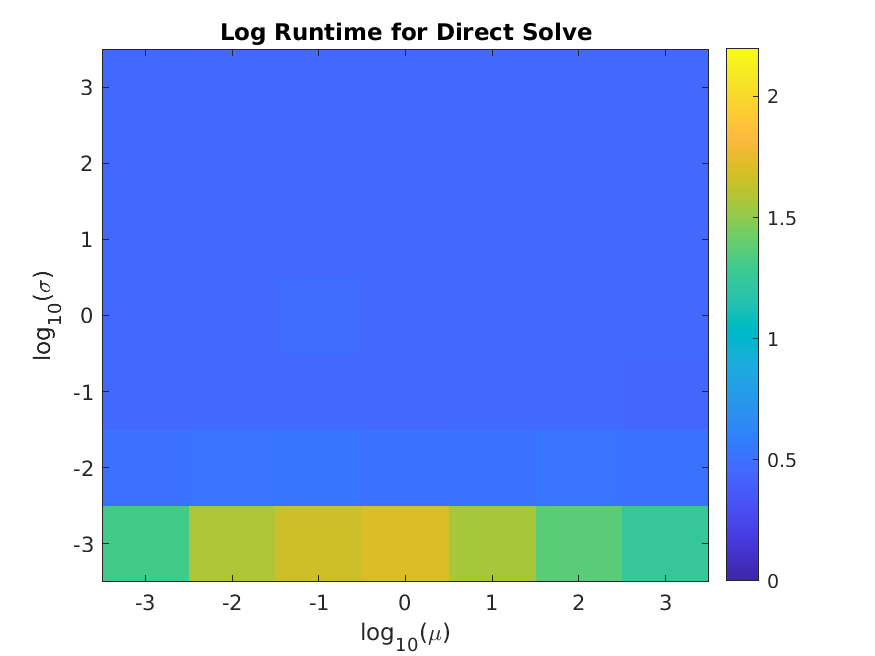
\includegraphics[width=\textwidth]{plots/dir1.png}
        \caption{Subfigure 1}
        \label{fig:sub1}
    \end{subfigure}
    \hfill
    \begin{subfigure}[t]{0.3\textwidth}
        \centering
        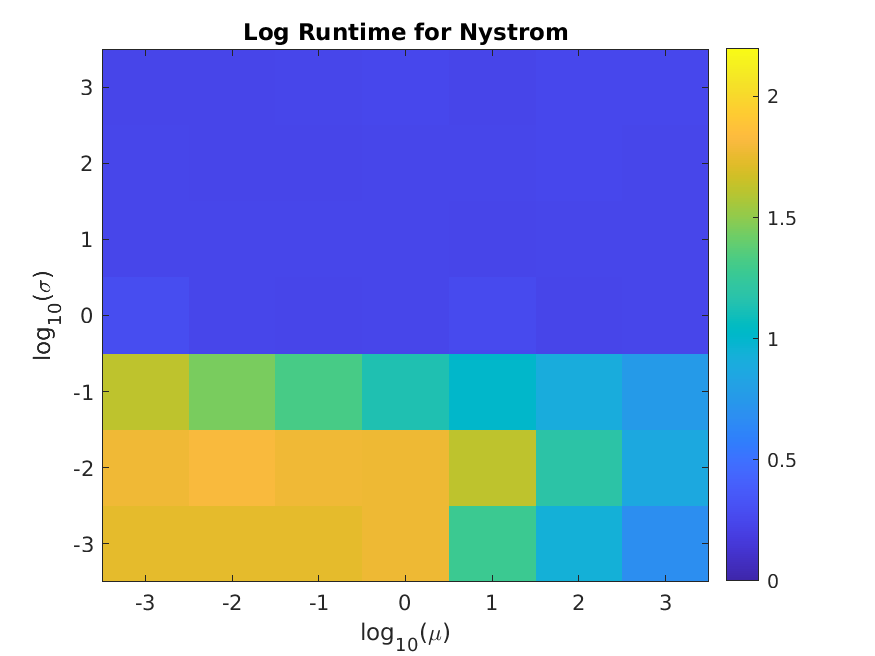
\includegraphics[width=\textwidth]{plots/nys1.png}
        \caption{Subfigure 2}
        \label{fig:sub2}
    \end{subfigure}
    \hfill
    \begin{subfigure}[t]{0.3\textwidth}
        \centering
        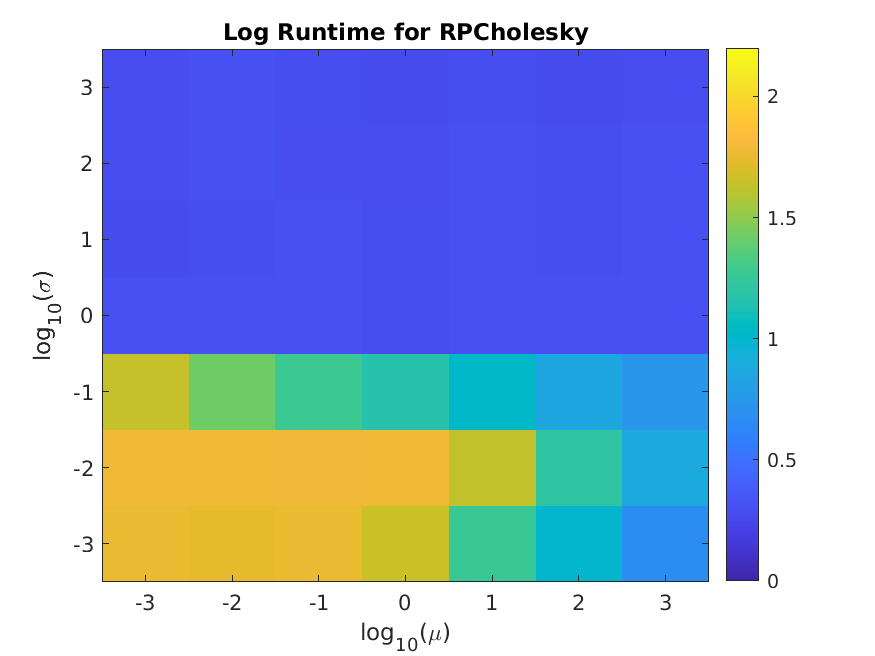
\includegraphics[width=\textwidth]{plots/rpc1.png}
        \caption{Subfigure 3}
        \label{fig:sub3}
    \end{subfigure}
    
    \vskip\baselineskip
    % Second row
    \begin{subfigure}[t]{0.3\textwidth}
        \centering
        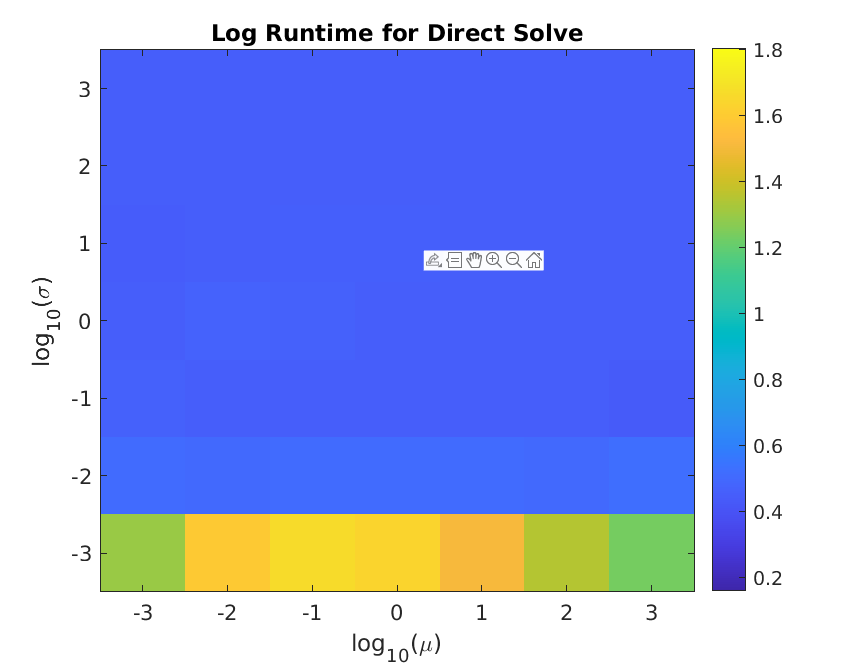
\includegraphics[width=\textwidth]{plots/dir2.png}
        \caption{Subfigure 4}
        \label{fig:sub4}
    \end{subfigure}
    \hfill
    \begin{subfigure}[t]{0.3\textwidth}
        \centering
        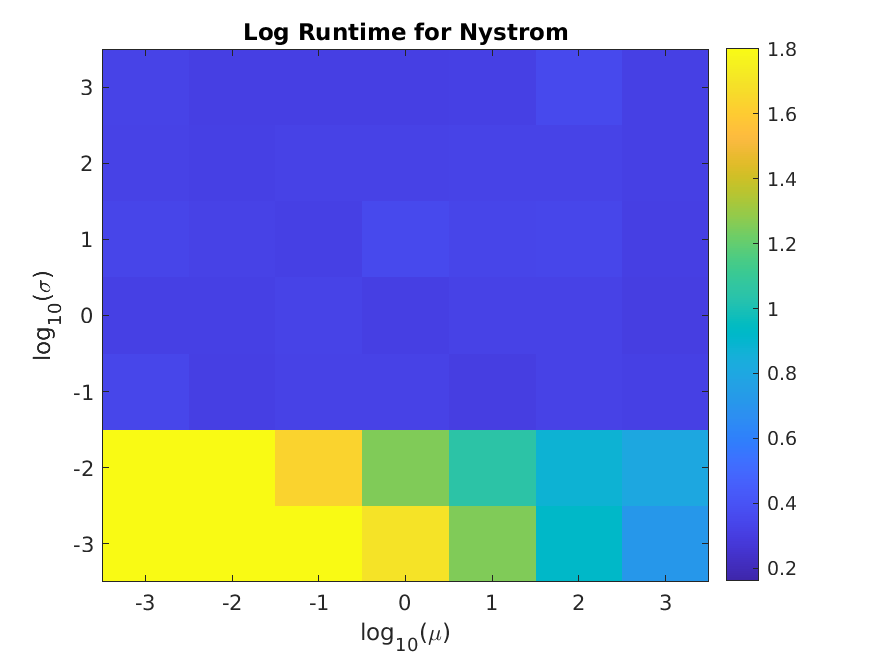
\includegraphics[width=\textwidth]{plots/nys2.png}
        \caption{Subfigure 5}
        \label{fig:sub5}
    \end{subfigure}
    \hfill
    \begin{subfigure}[t]{0.3\textwidth}
        \centering
        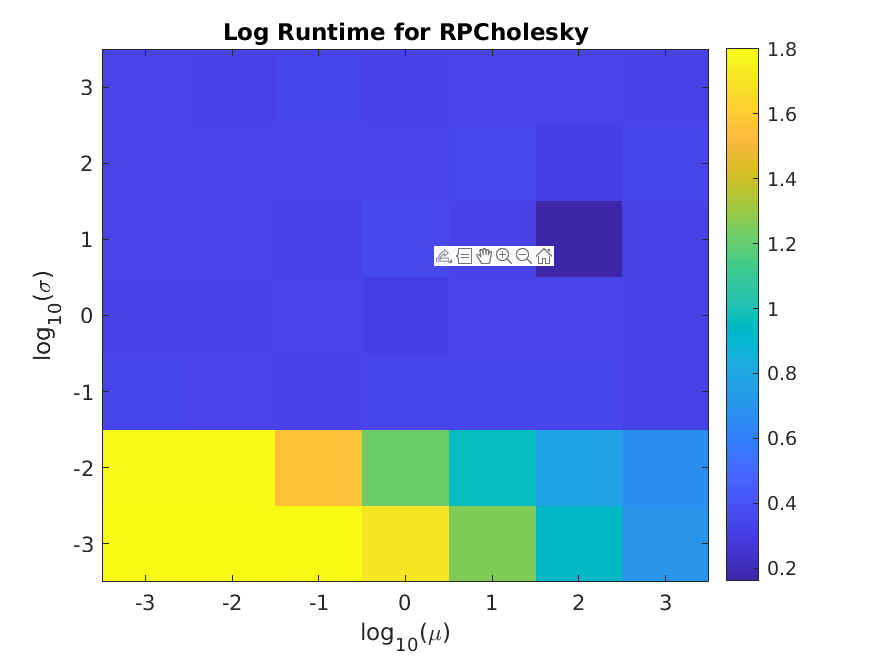
\includegraphics[width=\textwidth]{plots/rpc2.png}
        \caption{Subfigure 6}
        \label{fig:sub6}
    \end{subfigure}
    
    \vskip\baselineskip
    % Third row
    \begin{subfigure}[t]{0.3\textwidth}
        \centering
        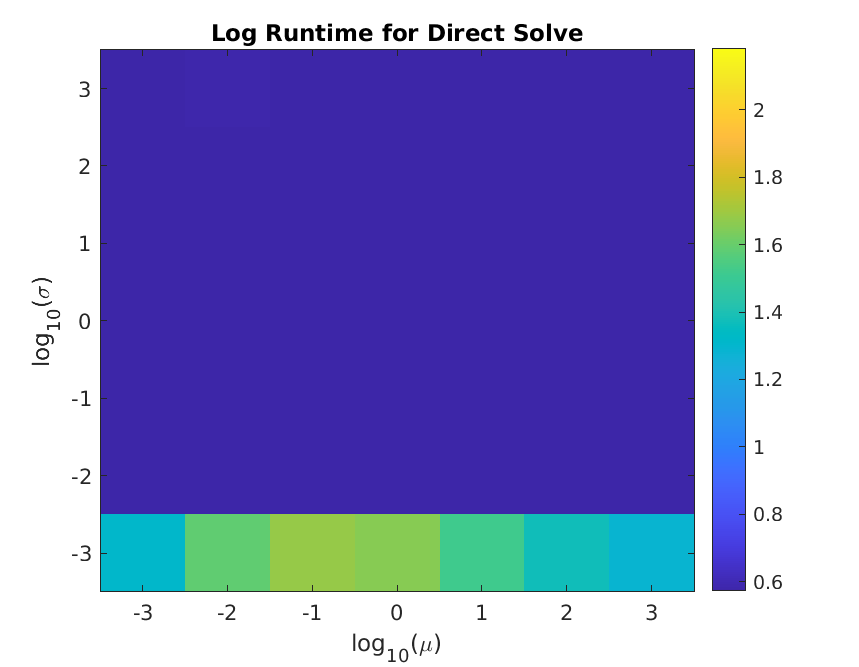
\includegraphics[width=\textwidth]{plots/dir3.png}
        \caption{Subfigure 7}
        \label{fig:sub7}
    \end{subfigure}
    \hfill
    \begin{subfigure}[t]{0.3\textwidth}
        \centering
        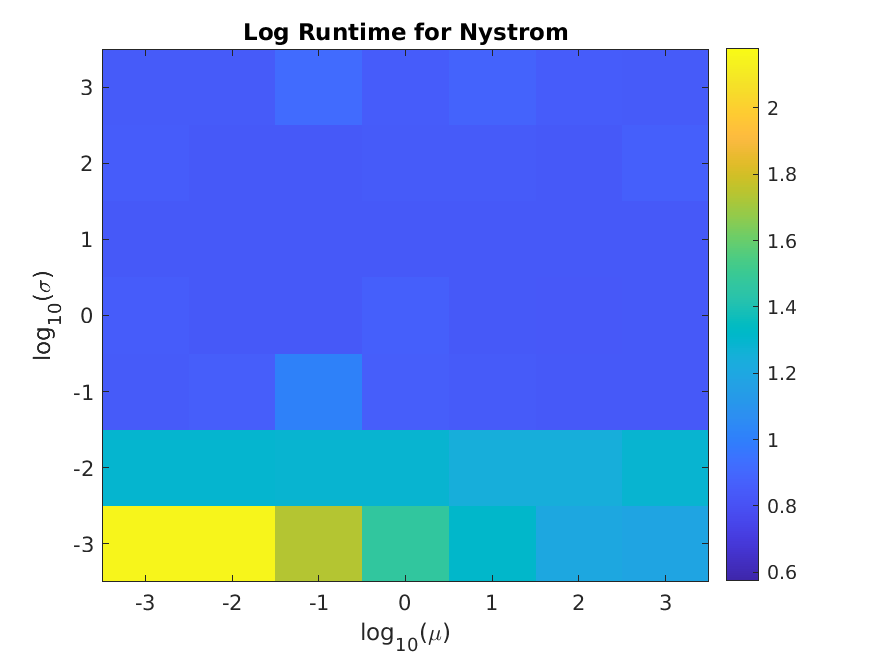
\includegraphics[width=\textwidth]{plots/nys3.png}
        \caption{Subfigure 8}
        \label{fig:sub8}
    \end{subfigure}
    \hfill
    \begin{subfigure}[t]{0.3\textwidth}
        \centering
        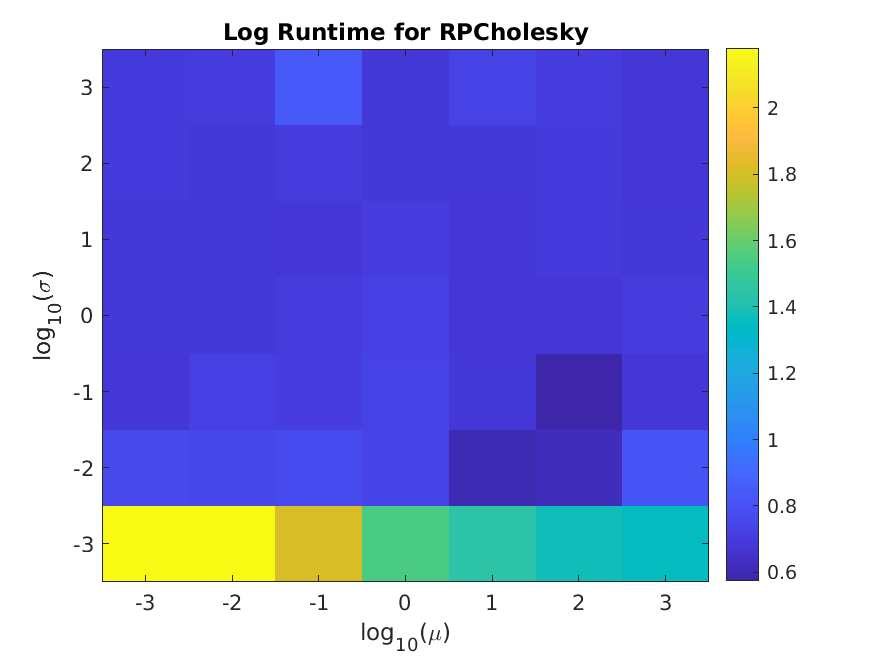
\includegraphics[width=\textwidth]{plots/rpc3.png}
        \caption{Subfigure 9}
        \label{fig:sub9}
    \end{subfigure}

    \caption{A 3x3 grid of subfigures.}
    \label{fig:grid}
\end{figure}

\end{enumerate}


\end{document}
